
%(BEGIN_QUESTION)
% Copyright 2012, Tony R. Kuphaldt, released under the Creative Commons Attribution License (v 1.0)
% This means you may do almost anything with this work of mine, so long as you give me proper credit

A {\it boiling-water reactor} (BWR) in a nuclear power plant uses the heat emitted by the nuclear ``core'' to boil water into steam, which is then used to turn a steam turbine and drive an electrical generator to produce electricity:

$$\includegraphics[width=15.5cm]{i01018x01.eps}$$

It is critically important that the nuclear core be kept completely submerged in water, lest it overheat. 

\vskip 10pt

Suppose the temperature and pressure measurements on a BWR are 780 $^{o}$F and 495 PSIG, respectively.  Reference a steam table and then determine whether the core is covered (submerged) or uncovered (exposed).

\underbar{file i01018}
%(END_QUESTION)





%(BEGIN_ANSWER)

The saturation temperature of steam at 505 PSIG (greater than 495 PSIG) is 471 $^{o}$F.  Since 780 $^{o}$F is much greater than this, we may deduce that the steam in the hot leg is superheated, and thus the core must be adding heat to the steam after it has boiled away from the water.  Thus, the core is uncovered.
 
\vskip 10pt

This is a very bad situation.

%(END_ANSWER)





%(BEGIN_NOTES)

During the Three Mile Island nuclear accident, two engineers from B\&W (Burt Dunn and Lou Carton) heard reports of the pressure and temperature readings at the ``hot leg'' pipe being 495 PSIG and over 600 $^{o}$F and concluded from these values that the reactor's core must have become uncovered (pages 40-41 of the report {\it Three Mile Island -- A Report to the Commissioners and to the Public, Volume I}).

%INDEX% Physics, heat and temperature: saturated steam pressure versus temperature
%INDEX% Physics, heat and temperature: steam table
%INDEX% Physics, heat and temperature: superheated steam

%(END_NOTES)


